\documentclass[12pt,twoside]{manual}

\pagestyle{plain}
\begin{document}






%%######################################################################
%% Styles
%%######################################################################

\tikzstyle{parentIsotope} = [rectangle, rounded corners, minimum width=3cm, minimum height=1cm,text centered, draw=black, fill=white]
\tikzstyle{unstableIsotope} = [rectangle, minimum width=3cm, minimum height=1cm,text centered, draw=black, fill=white]
\tikzstyle{stableIsotope} = [rectangle, rounded corners, minimum width=3cm, minimum height=1cm,text centered, draw=black, fill=white]
\tikzstyle{isotopeProduction} = [rectangle, minimum width=3cm, minimum height=1cm,text centered, draw=black, fill=white]








%%######################################################################
%% Listings
%%######################################################################

\lstdefinestyle{inputfile}
{
  breaklines=true,
  numbers=left,
  stepnumber=1,
  tabsize=4,
  numberstyle=\tiny\color{gray},
  keywordstyle=\color{blue},
  commentstyle=\color{dkgreen},
  stringstyle=\color{mauve}
}

\lstdefinestyle{spython}
{
	language=Python,
  breaklines=true,
  numbers=left,
  stepnumber=1,
  tabsize=4,
  numberstyle=\tiny\color{gray},
  keywordstyle=\color{blue},
  commentstyle=\color{dkgreen},
  stringstyle=\color{mauve}
}


%%######################################################################
%% Cover Page
%%######################################################################

\begin{titlepage}
  \begin{center}
    \centerline{
\includegraphics[width=0.7\textwidth]{img/coverart}}


    \textbf{Department of Metallurgy \& Materials}

    \vspace*{2.0cm}
    \Large{}
    \textbf{Activity V2 Manual}
    \vspace{0.8cm}
    \normalsize{}

  \end{center}
\end{titlepage}

\pagenumbering{gobble}

\pagenumbering{roman} 

\tableofcontents

\pagenumbering{arabic}




%%######################################################################
%% Overview
%%######################################################################

\chapter{Overview}

\section{Reason for the Program}

The Activity program calculates how radioactive a target becomes after being irradiated by high energy ions.  It uses the TENDL-2019\cite{tendl2019} database that contains cross-section data for protons and deuterons, and the JEFF-3.3 Radioactive Decay Data File\cite{jeff33}.

\section{Program Requirements}

The user must provide a exyz file from the SRIM\cite{srim} ion transport program and a breakdown of the composition of the target, as well as other irradiation parameters.



%%######################################################################
%% Installation
%%######################################################################

\chapter{Installation}

The program needs Python 3 installed in order to run.  At the time of writing, it has only been developed to run on a Linux operating system, but it shouldn't require much adjusting to run on a Windows computer too.

Download and install the latest version of Python 3:

https://www.python.org/downloads

The latest version of the activity code with data files must also be downloaded:

https://github.com/BenPalmer1983/activity\_v2

For example, I have installed to /home/ben/activity

\FloatBarrier

\begin{figure}[h]
  \begin{center}
    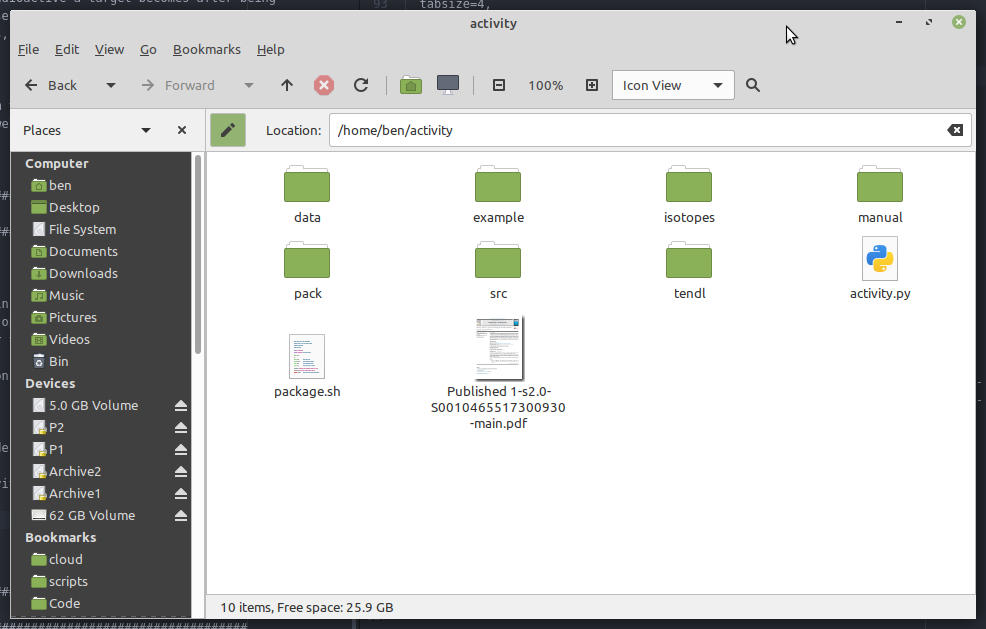
\includegraphics[scale=0.50]{img/installdir}
  \end{center}
\end{figure}



\FloatBarrier

%%######################################################################
%% How to Use
%%######################################################################

\chapter{How To Use}


\section{SRIM}

If you haven't done so already, run the required simulation in SRIM.  When setting up the calculation, be sure to set an increment for the EXYZ file.  Sane values that have been used in examples range from 10eV to 10,000KeV, but this will depend on the resolution of the data in the TENDL database, the thickness of your target and the energy of the projectiles.

\FloatBarrier

\begin{figure}[h]
  \begin{center}
    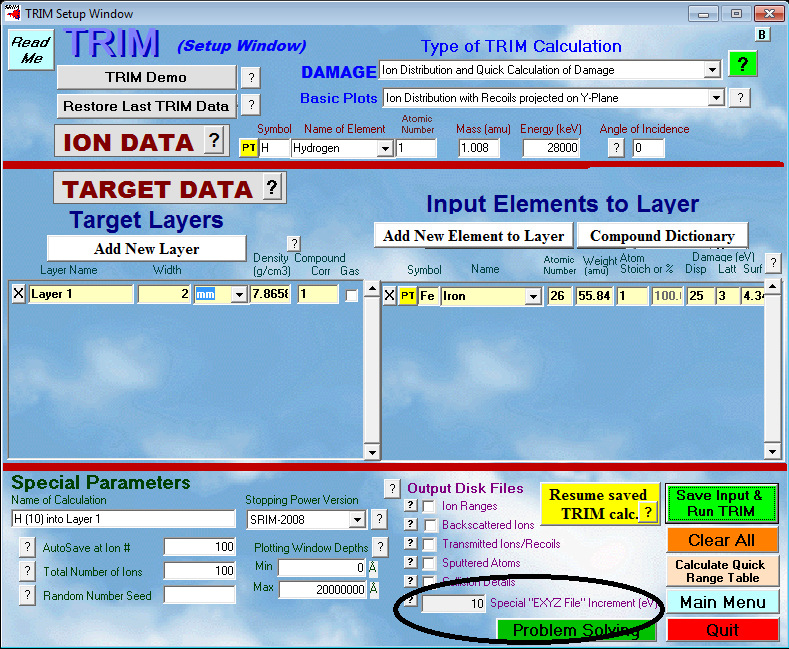
\includegraphics[scale=0.50]{img/srim1}
  \end{center}
\end{figure}

\begin{figure}[h]
  \begin{center}
    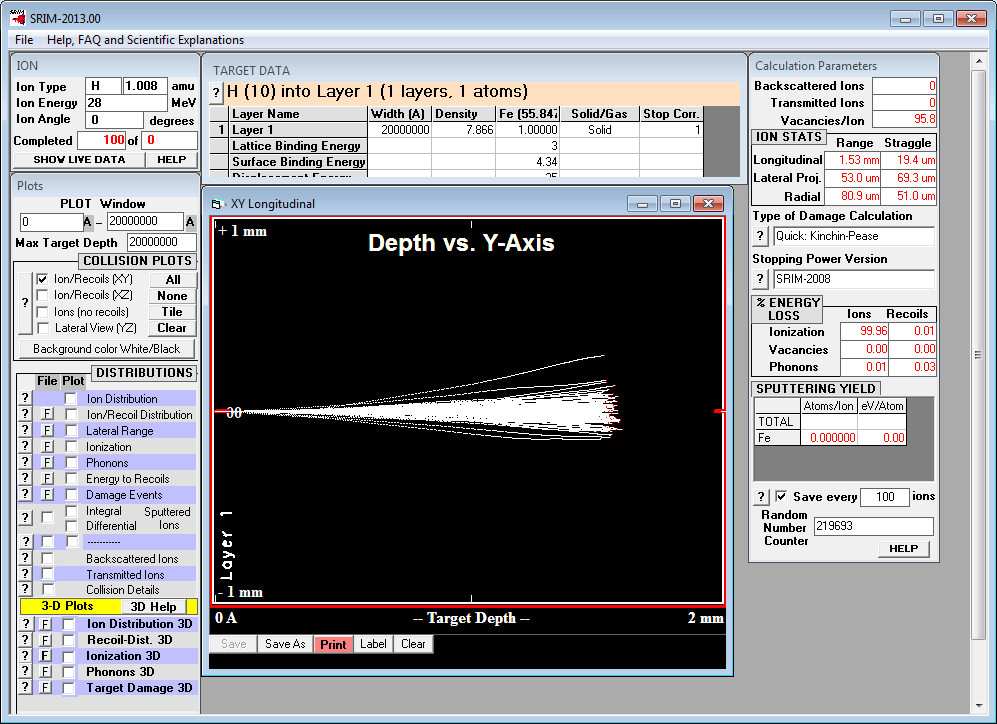
\includegraphics[scale=0.40]{img/srim2}
  \end{center}
\end{figure}

\begin{figure}[h]
  \begin{center}
    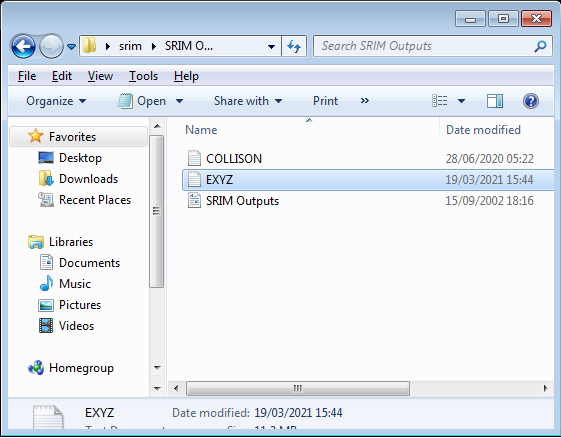
\includegraphics[scale=0.60]{img/srim3}
  \end{center}
\end{figure}

\FloatBarrier

Take a copy of the EXYZ.txt file as it will be required by the activity program.

\section{Activity}

Create a directory to run the calculation.  Copy in the EXYZ.txt file and create an input file.


  \begin{center}
    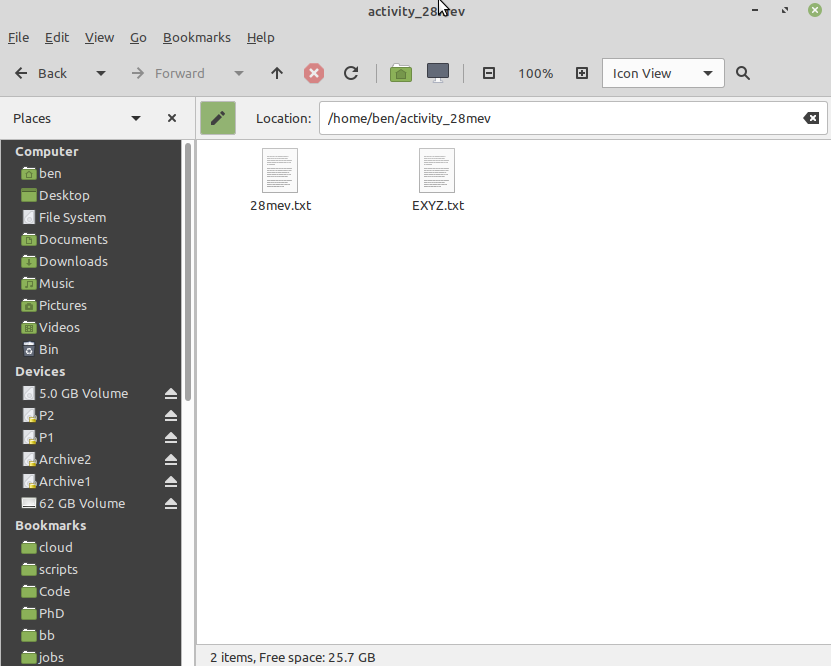
\includegraphics[scale=0.40]{img/activityexample1}
  \end{center}


The input file is just a text file, and will specify the calculation details.  The data file paths must be specified, and then the simulations can be detailed, each with it's own unique name.  The example below is for two simulations - the first with a 300s beam, and the second with a 3000s beam.



\FloatBarrier

\begin{lstlisting}[style=inputfile, caption={}]
# Data files
data isotopes="/home/ben/activity/data/isotopes" xs="/home/ben/activity/data/xs"

# Sim 1
sim1 exyz="EXYZ.txt" target_composition=Fe,100.0 target_depth=0.5,mm target_density=7808,kgm3 beam_projectile='proton' beam_energy=28,MeV beam_area=64,mm2 beam_duration=300,s beam_current=0.5,uA end_time=260000,s

# Sim 2
sim2 exyz="EXYZ.txt" target_composition=Fe,100.0 target_depth=0.5,mm target_density=7808,kgm3 beam_projectile='proton' beam_energy=28,MeV beam_area=64,mm2 beam_duration=3000,s beam_current=5.0,uA end_time=260000,s
\end{lstlisting}

\FloatBarrier

The program is run from the terminal/command line.  Depending on your computer system, python3 might run through the command python3 or python, and on my computer the command is python3.

\begin{lstlisting}[style=inputfile, caption={}]
python3 /home/ben/activity/activity.py /home/ben/activity_28mev/28mev.txt
\end{lstlisting}

\FloatBarrier

The program outputs into a directory for each simulation.

\begin{figure}[h]
  \begin{center}
    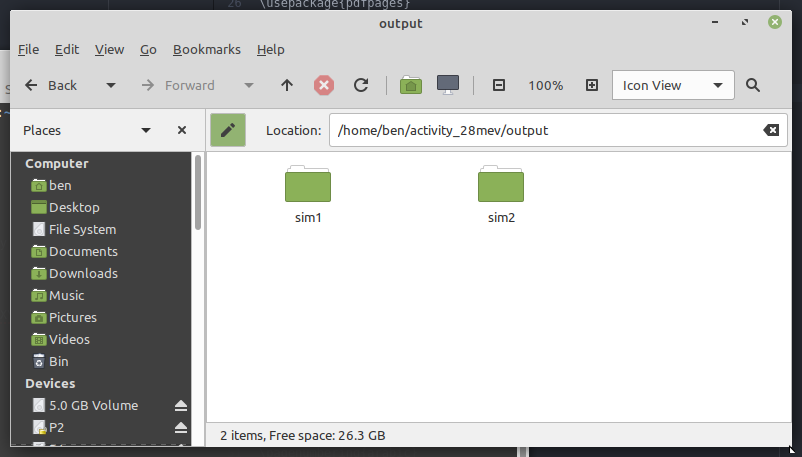
\includegraphics[scale=0.30]{img/output1}
  \end{center}
\end{figure}

\begin{figure}[h]
  \begin{center}
    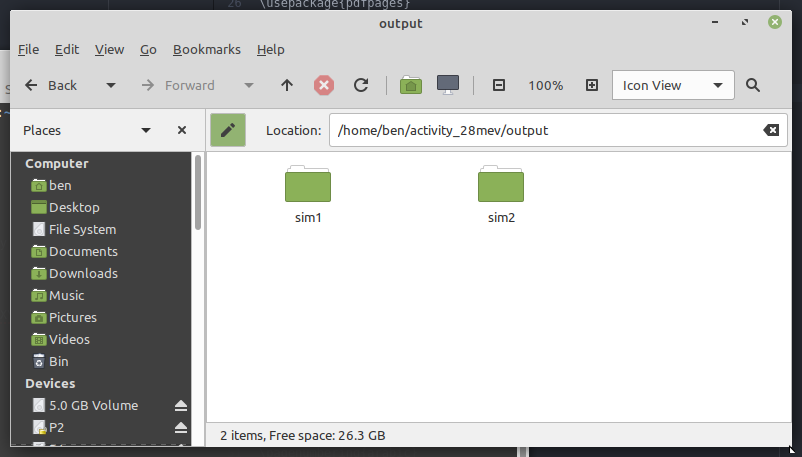
\includegraphics[scale=0.30]{img/output1}
  \end{center}
\end{figure}

\FloatBarrier

Within each directory are various plots and data files, including the activity over time and predicted gamma lines.

\FloatBarrier

\begin{figure}[h]
  \begin{center}
    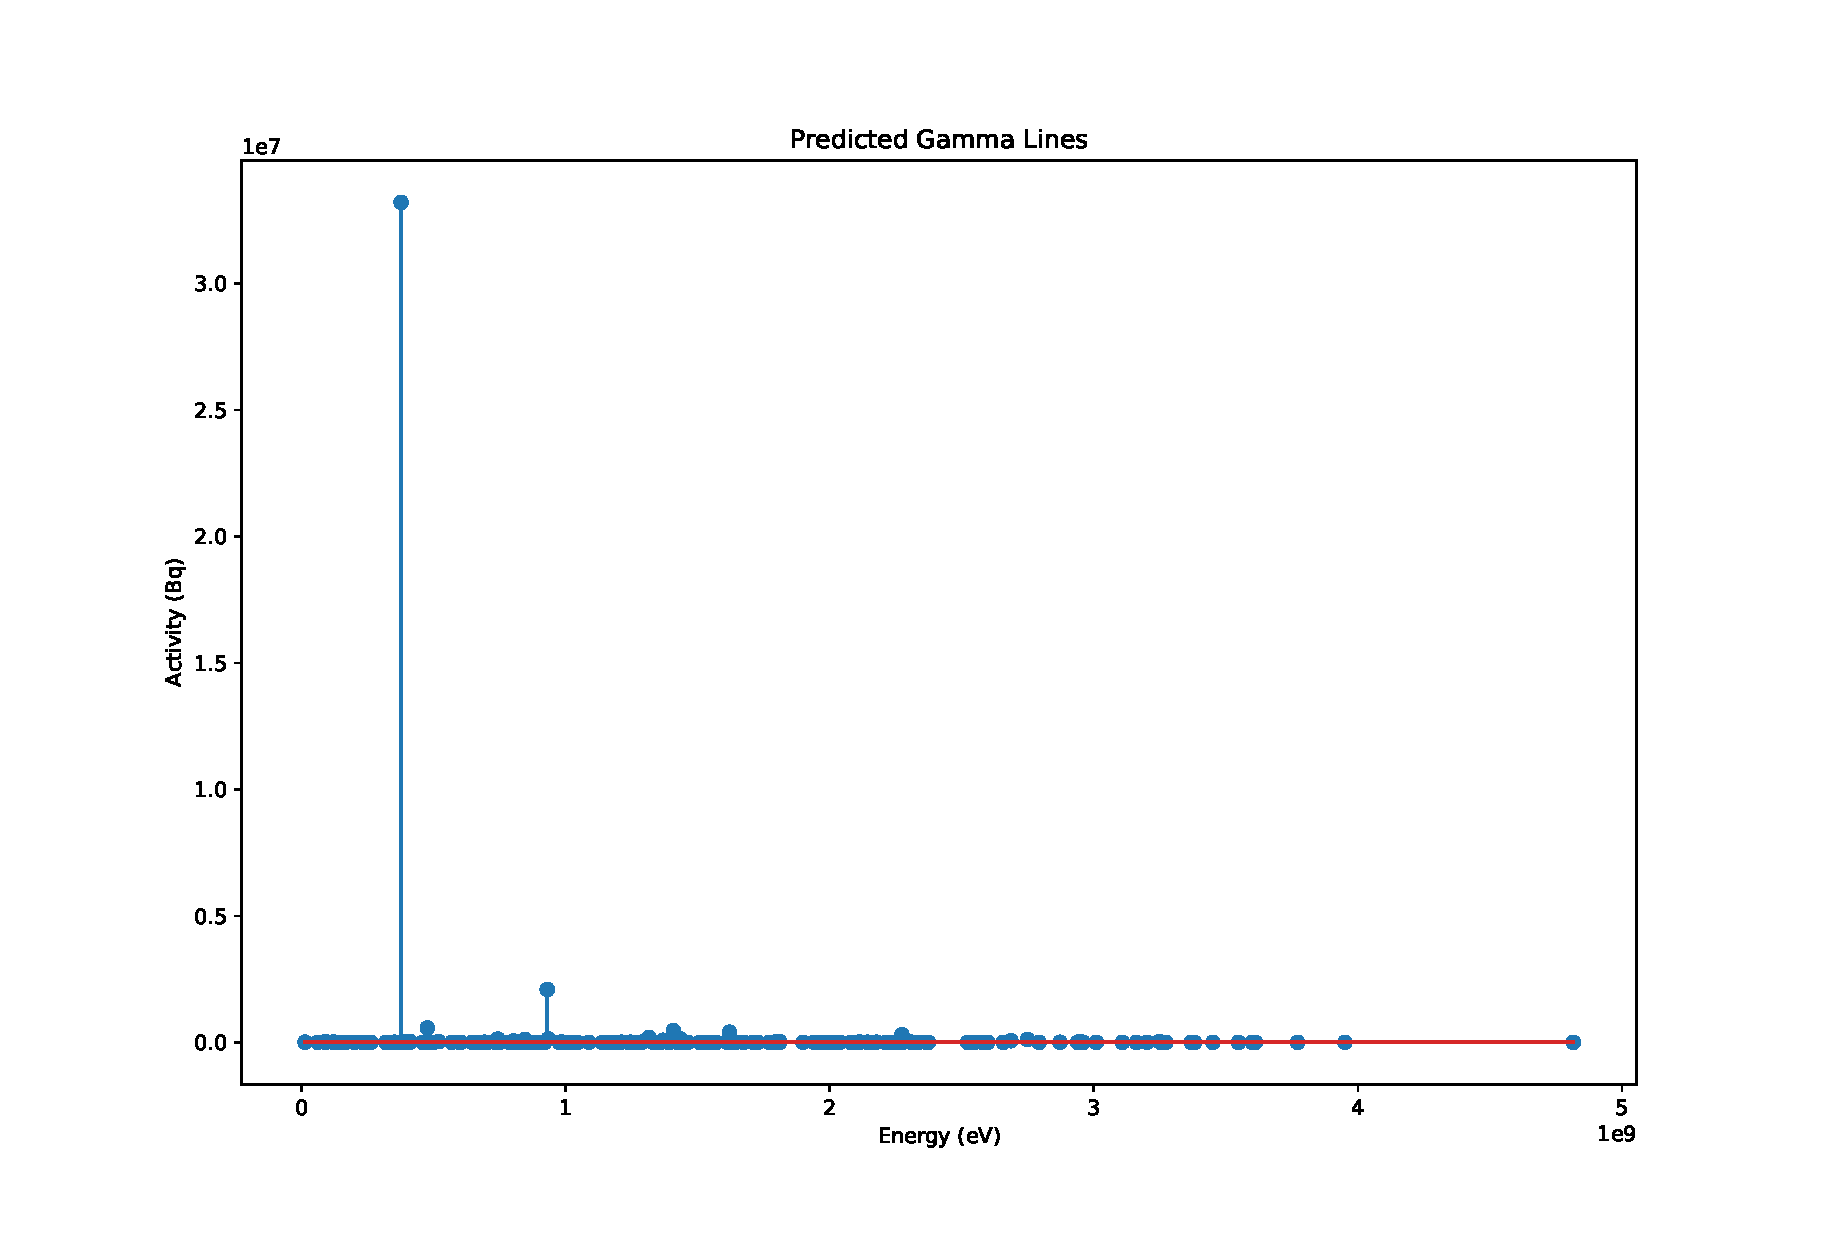
\includegraphics[scale=0.25]{img/end_of_beam_gamma_lines.eps}
  \end{center}
\end{figure}

\begin{figure}[h]
  \begin{center}
    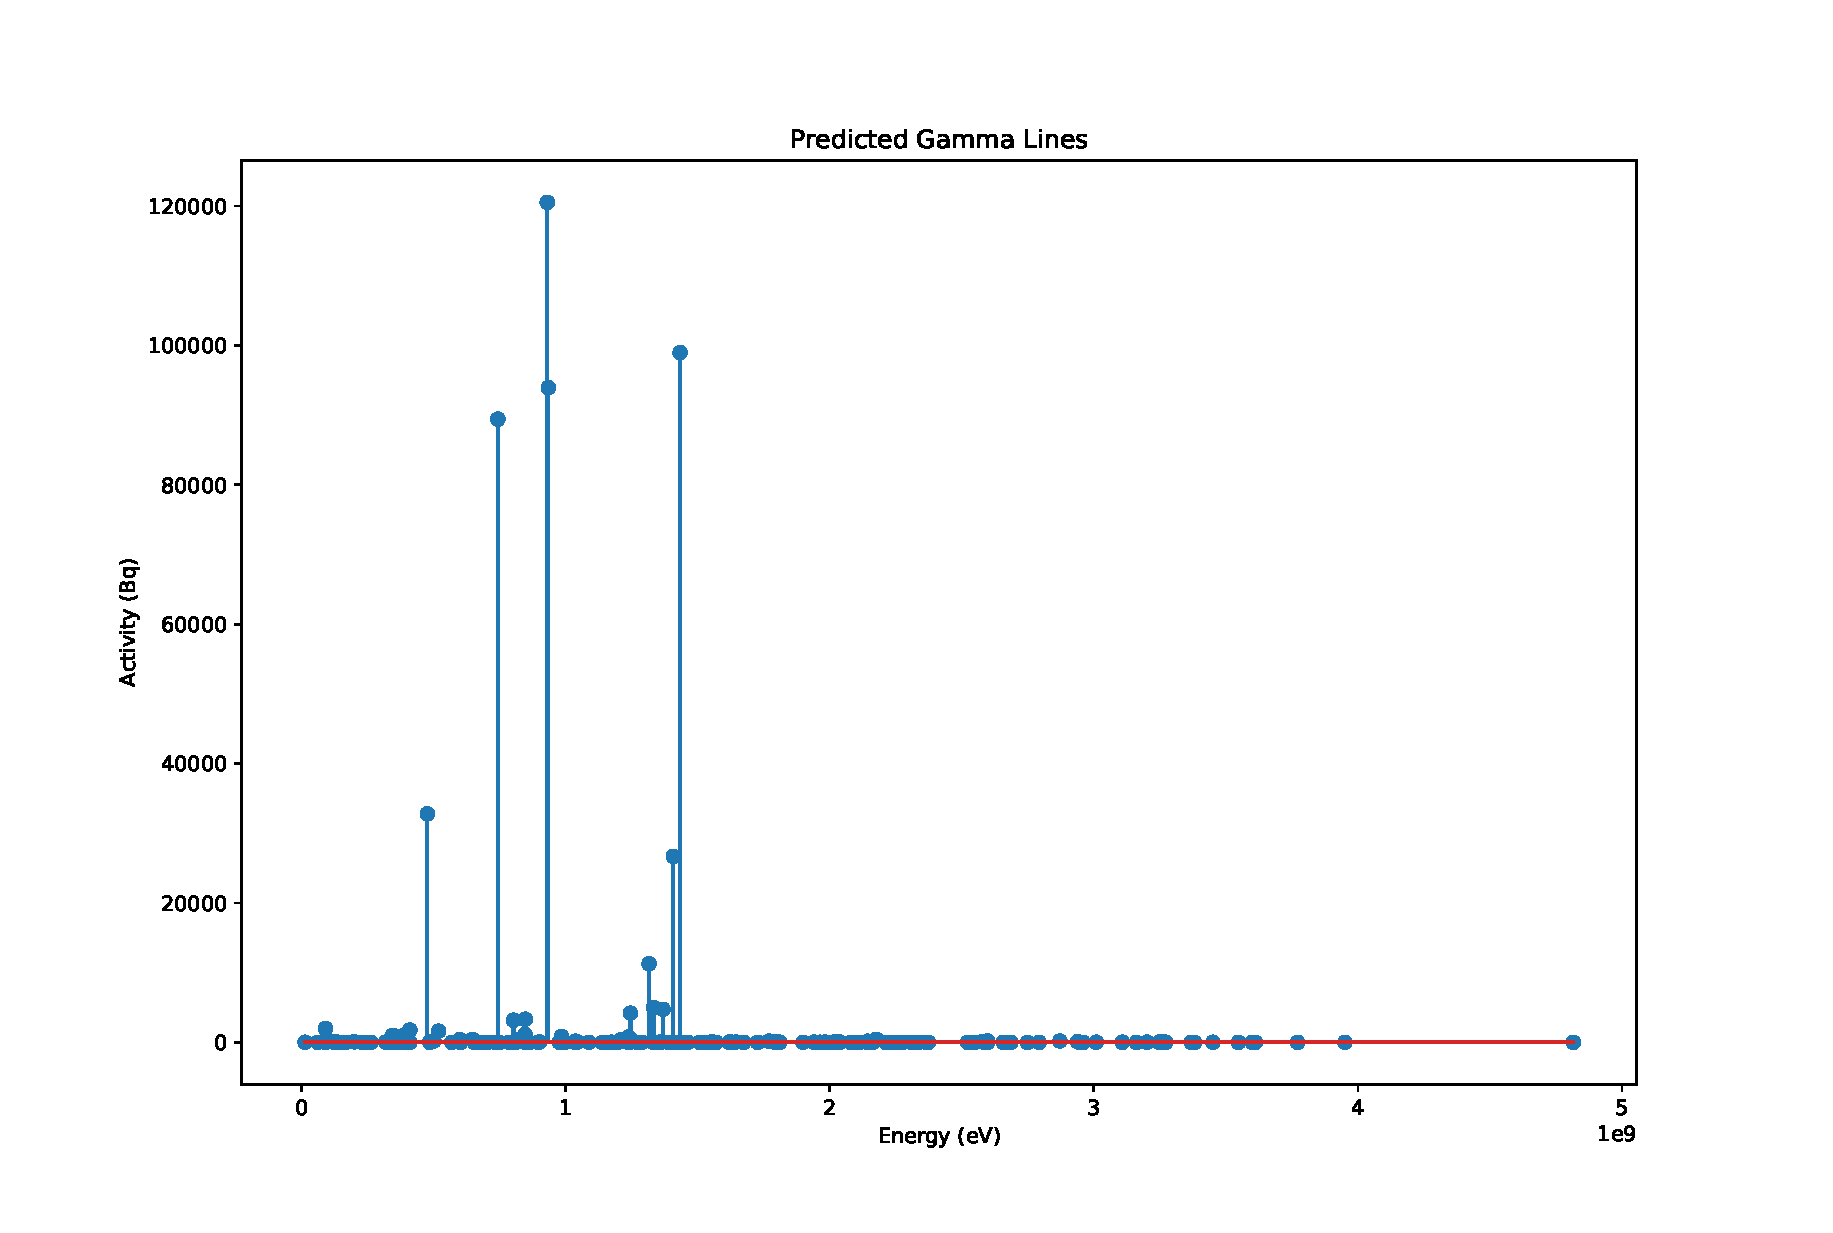
\includegraphics[scale=0.25]{img/end_of_sim_gamma_lines.eps}
  \end{center}
\end{figure}

\begin{figure}[h]
  \begin{center}
    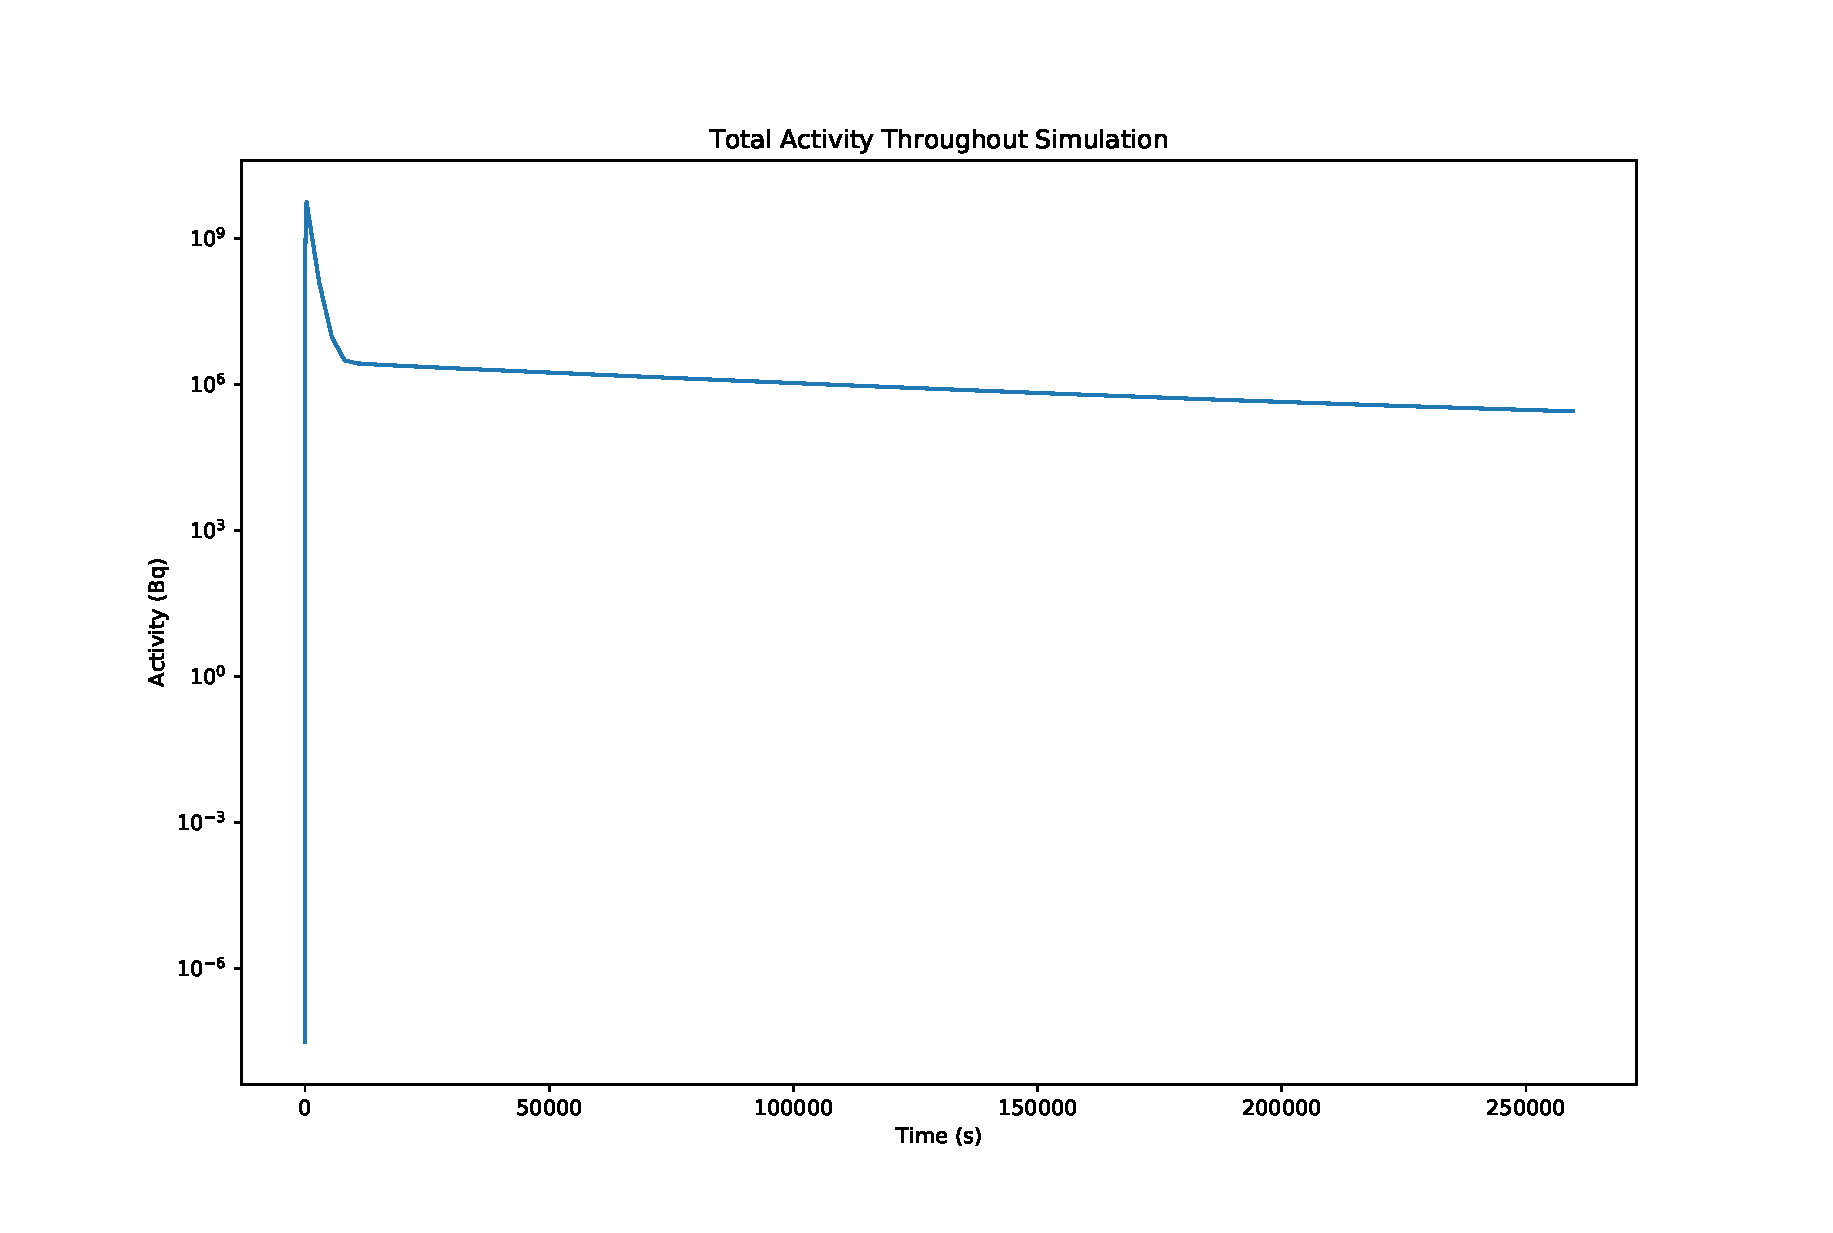
\includegraphics[scale=0.25]{img/total_sim_total_activity_log.eps}
  \end{center}
\end{figure}


\FloatBarrier

The program analyses the exyz file and output a chart showing the distribution of energy lost by projectiles as they pass through the target.  

\begin{figure}[h]
  \begin{center}
    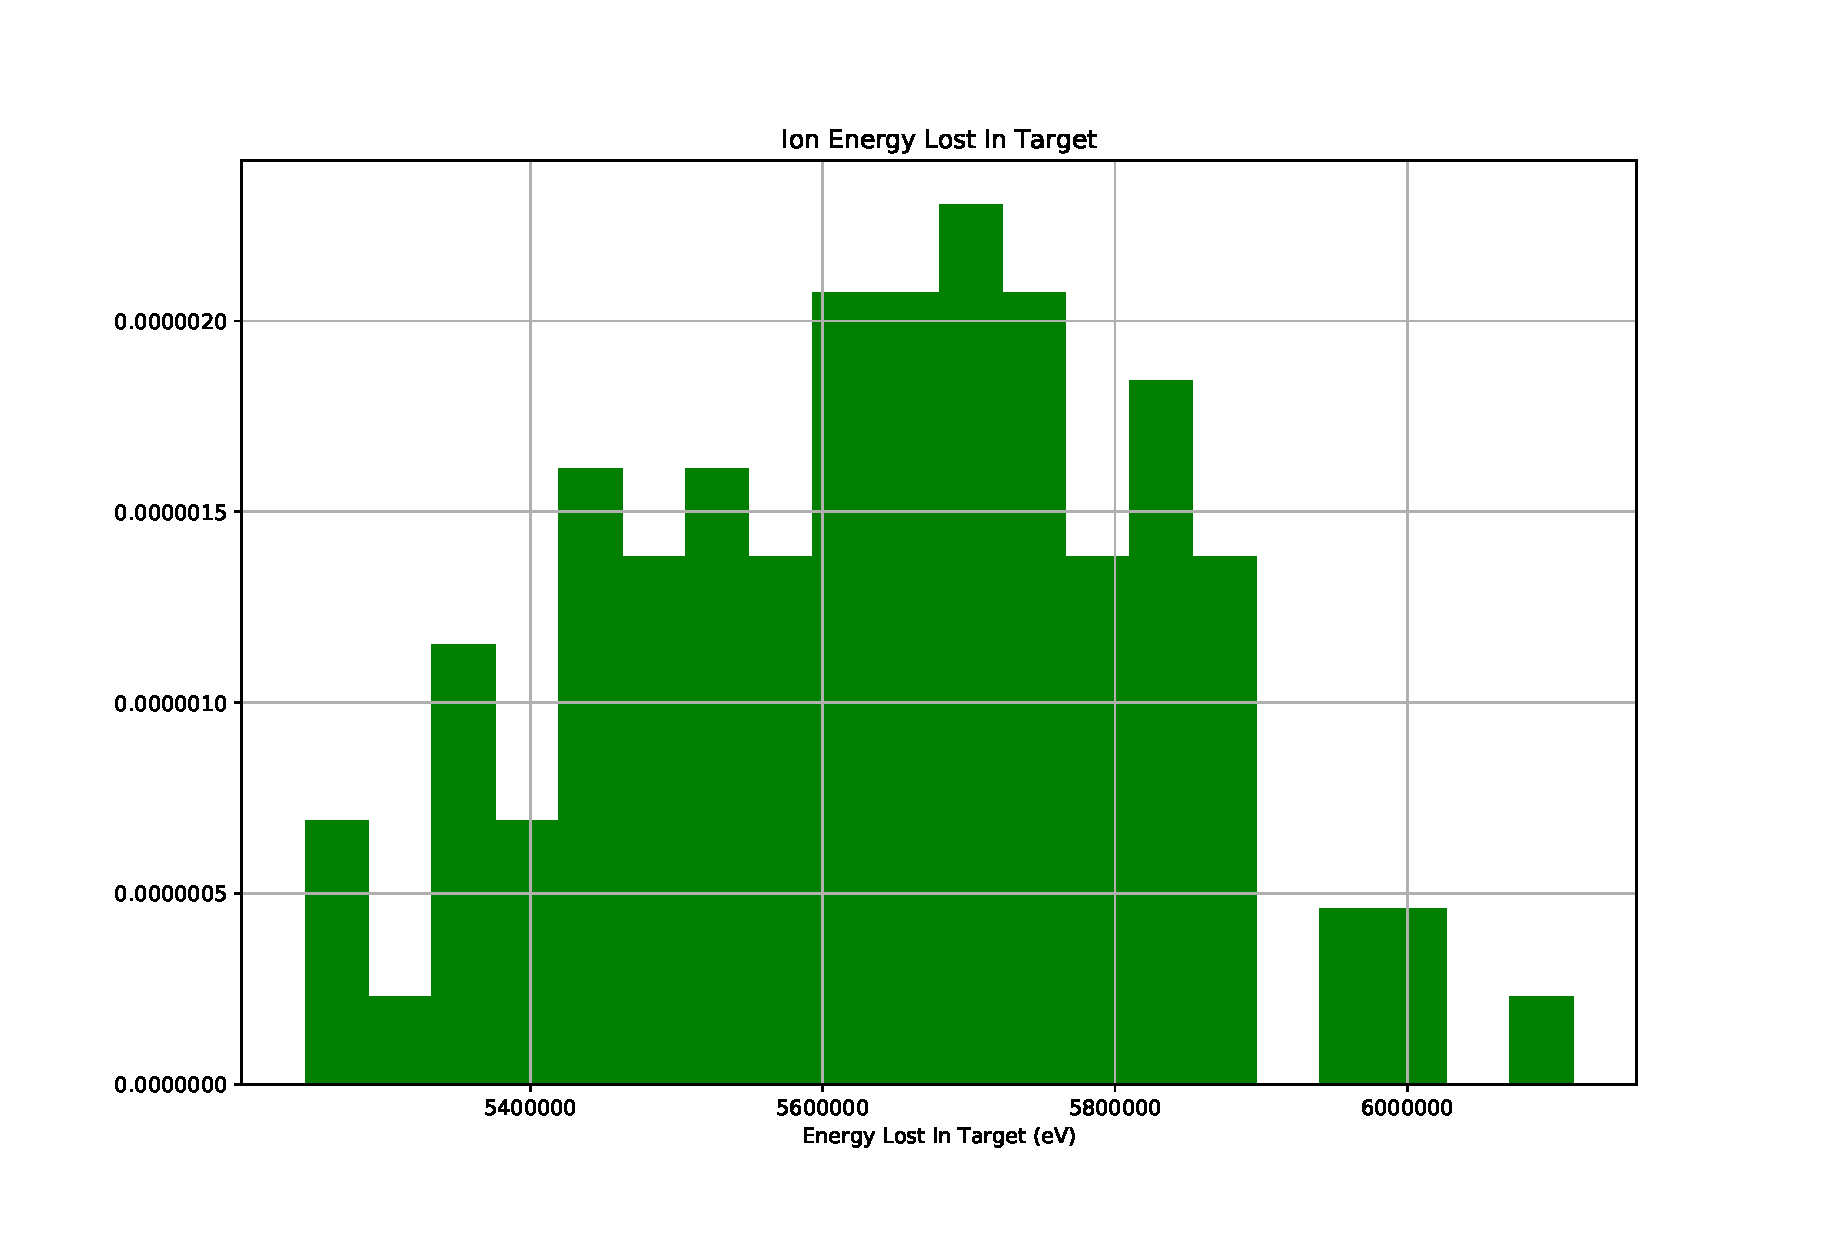
\includegraphics[scale=0.25]{img/ion_energy_lost.eps}
  \end{center}
\end{figure}

As a target is irradiated, the residual radioactive isotopes begin to decay.  To begin with, the production outweighs the decay, but at a certain point there's enough of the radioactive isotope within the target that the decay balances with the production.  At this point the radioactive isotope in the target is saturated, and will not increase above this amount unless the beam parameters are adjusted.

The saturation times depend on the isotope and the various reaction cross sections with the projectile.  The saturation plots for each radioactive isotope are created and saved by the program.

\begin{figure}[h]
  \begin{center}
    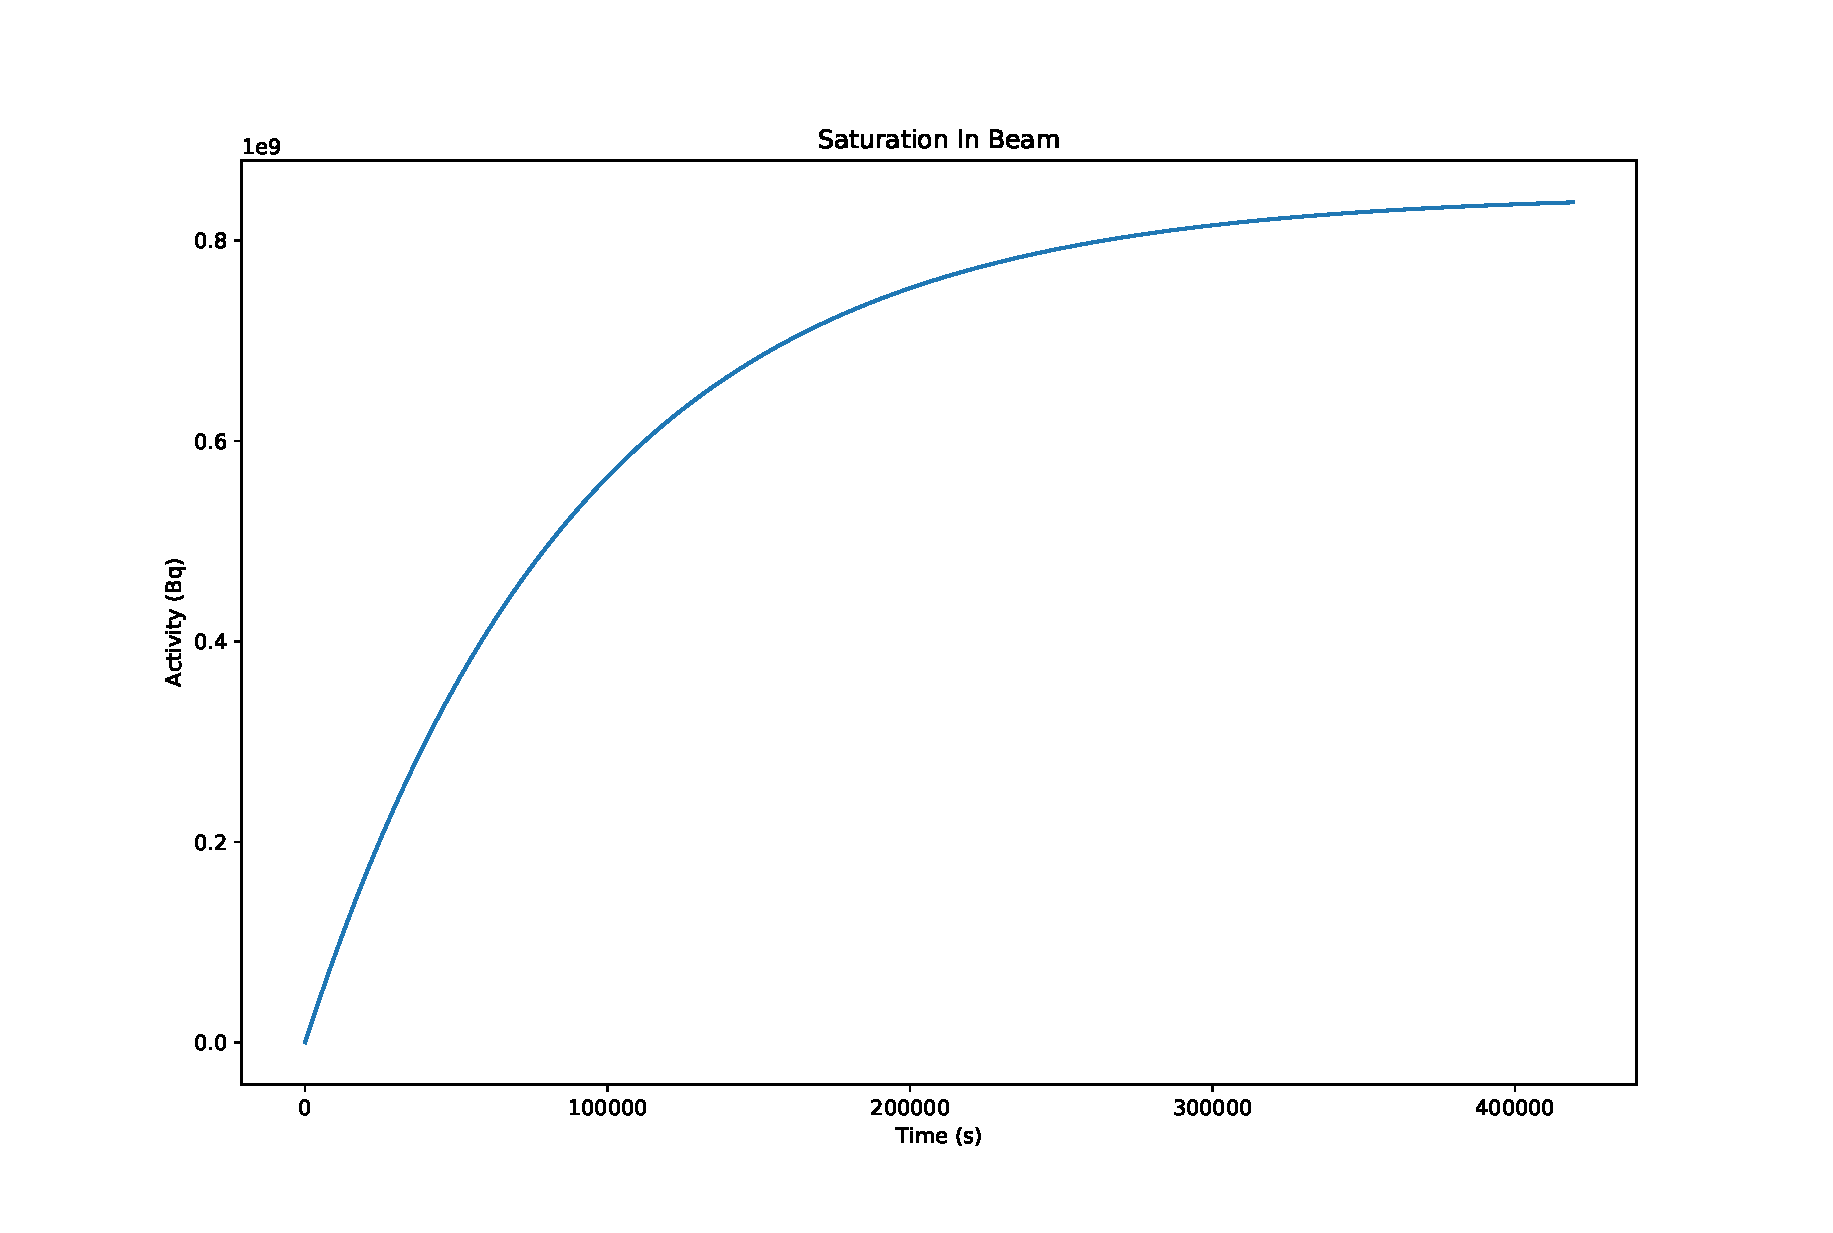
\includegraphics[scale=0.25]{img/saturation_Co55.eps}
  \end{center}
  \caption{Saturation of Cobalt-55}
\end{figure}

\begin{figure}[h]
  \begin{center}
    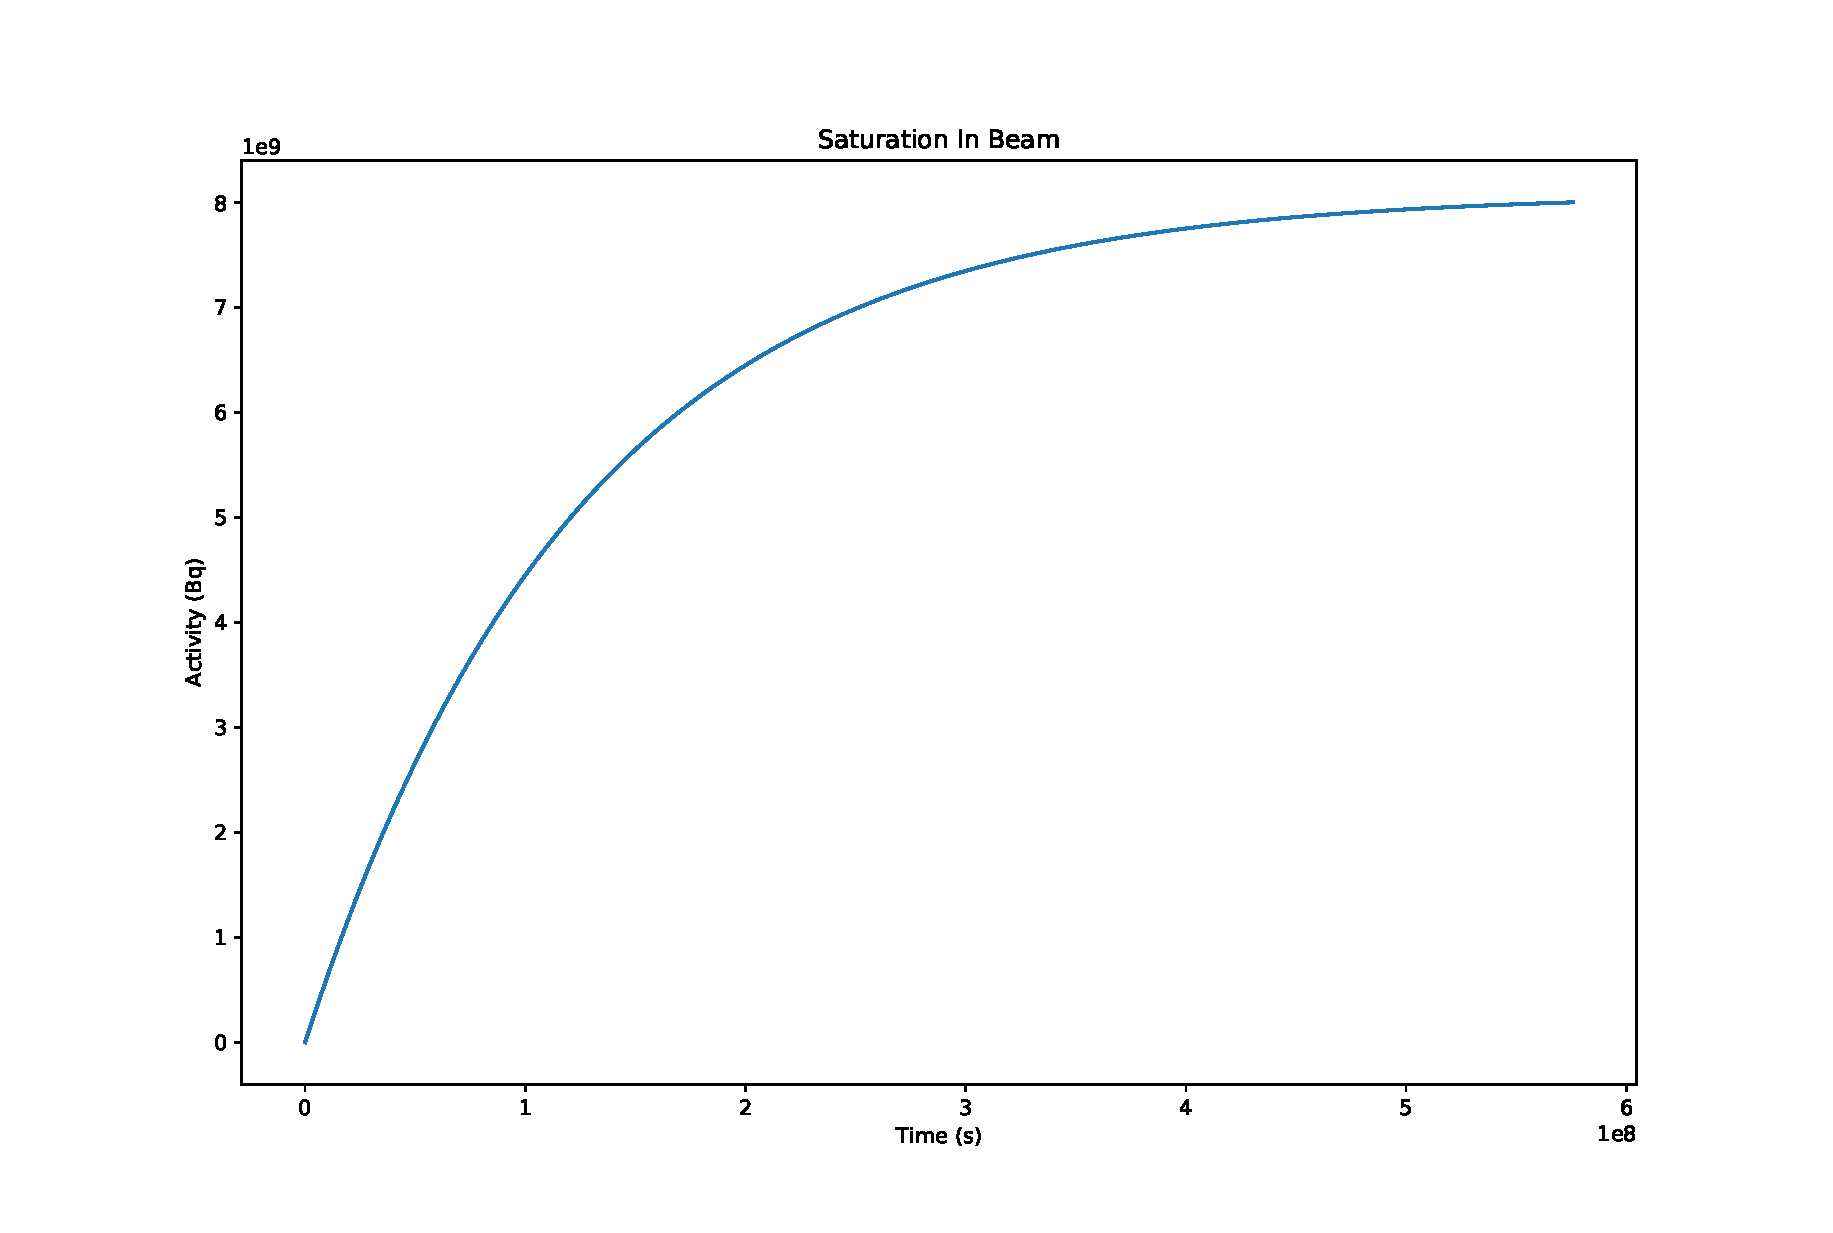
\includegraphics[scale=0.25]{img/saturation_Fe55.eps}
  \end{center}
  \caption{Saturation of Iron-55}
\end{figure}


\FloatBarrier

%%######################################################################
%% Examples
%%######################################################################

\chapter{Examples}

\section{Iron - 28MeV Protons}

In this example, natural iron makes up the target . 

\begin{lstlisting}[style=inputfile, caption={}]
# Data files
data isotopes="/home/ben/activity/data/isotopes" xs="/home/ben/activity/data/xs"

# Sim
sim1 exyz="EXYZ.txt" target_composition=Fe,100.0 target_depth=0.5,mm target_density=7808,kgm3 beam_projectile='proton' beam_energy=28,MeV beam_area=64,mm2 beam_duration=300,s beam_current=0.5,uA end_time=260000,s
\end{lstlisting}

The simulation section defines what the target material is made of as well as the beam parameters.  



\section{Iron Fe56 (only) - 28MeV Protons}

In this example, the target is made of Fe56 only, and contains none of the other naturally occurring stable isotopes.

\begin{lstlisting}[style=inputfile, caption={}]
# Data files
data isotopes="/home/ben/activity/data/isotopes" xs="/home/ben/activity/data/xs"

# Sim
sim1 exyz="EXYZ.txt" target_composition=Fe56,100.0 target_depth=0.5,mm target_density=7808,kgm3 beam_projectile='proton' beam_energy=28,MeV beam_area=64,mm2 beam_duration=300,s beam_current=0.5,uA end_time=260000,s
\end{lstlisting}



\section{Steel - 5MeV Protons}

This example was provided by Alex Dickinson-Lomas, with a steel containing a wider range of elements.

\begin{lstlisting}[style=inputfile, caption={}]
# Data files
data isotopes="/home/ben/activity/data/isotopes" xs="/home/ben/activity/data/xs"

# Sim
sim1 exyz="EXYZ.txt" target_composition=Fe,96.375,C,0.772,Cu,0.024,Mn,1.36,Ni,0.698,Si,0.381,Cr,0.092,V,0.008,P,0.009,Si,0.003,Mo,0.278 target_depth=0.1,mm target_density=7808,kgm3 beam_projectile='proton' beam_energy=5,MeV beam_area=64,mm2 beam_duration=300,s beam_current=0.5,uA end_time=260000,s
\end{lstlisting}









%%######################################################################
%% Decay Equation
%%######################################################################


\chapter{Decay Equation}

\section{Bateman Equation}


The Bateman equation was derived using Laplace transforms, and this same method has been used to develop a modified equation that incorporates branching factors and production rates for each isotope in the decay chain, as illustrated by Figure \ref{fig:decaytree}.


\begin{figure}[!h]
	\centering
	\begin{tikzpicture}[node distance=2cm]

	% Row 1
	\node (parent) [startstop] {Parent Isotope};
	\node (parent_source) [process, left of=parent, xshift=-4cm] {Parent Source};
	% Row 2
	\node (parent_branch) [decision, below of=parent] {Branching};
	% Row 3
	\node (daughter_1a) [process, below of=parent_branch, xshift=-2.5cm] {Daughter 1 (Branch A)};
	\node (daughter_1a_src) [process, left of=daughter_1a, xshift=-2.5cm] {External Source};
	\node (daughter_1b) [process, below of=parent_branch, xshift=2.5cm] {Daughter 1 (Branch B)};
	\node (daughter_1b_src) [process, right of=daughter_1b, xshift=2.5cm] {External Source};
	% Row 4
	\node (daughter_1a_branch) [decision, below of=daughter_1a, xshift=0.5cm] {Branching};
	% Row 5
	\node (daughter_2a) [process, below of=daughter_1a_branch, xshift=-0.5cm] {Daughter 2 (Branch A)};
	\node (daughter_2a_src) [process, left of=daughter_2a, xshift=-2.5cm] {External Source};
	\node (daughter_2b) [process, below of=daughter_1a_branch, xshift=4.5cm] {Daughter 2 (Branch B)};
	\node (daughter_2b_src) [process, right of=daughter_2b, xshift=2.5cm] {External Source};
	
	% arrows
	\draw [thick,->] (parent_source) -- (parent);
	\draw [thick,->] (parent) -- (parent_branch);
	\draw [thick,->] (parent_branch) -- (daughter_1a);
	\draw [thick,->] (parent_branch) -- (daughter_1b);
	\draw [thick,->] (daughter_1a_src) -- (daughter_1a);
	\draw [thick,->] (daughter_1b_src) -- (daughter_1b);
	\draw [thick,->] (daughter_1a) -- (daughter_1a_branch);
	\draw [thick,->] (daughter_1a_branch) -- (daughter_2a);
	\draw [thick,->] (daughter_1a_branch) -- (daughter_2b);
	\draw [thick,->] (daughter_2a_src) -- (daughter_2a);
	\draw [thick,->] (daughter_2b_src) -- (daughter_2b);
	
	%\draw [->] (isotope1) -- (isotope2);
	%\draw [->] (isotope2) -- (stable);


	\end{tikzpicture}
	\captionsetup{font={it}}
	\caption{An example of several decay chains including branching factors and possible external source terms for each isotope on each chain.}
	\label{fig:decaytree}
\end{figure}


\subsection{Laplace Transform}

Laplace Transforms (\ref{eq:eqLaplaceTransform}) are a useful mathematical tool, and allow ordinary differential equations to be solved by simple algebraic manipulation in the s domain.  Bateman took advantage of Laplace Transforms in deriving his equation, and this is the method that has been taken here as well.

\begin{equation}
  F(s) = \int \limits_{0}^{\infty} f(t) \exp(-st) dt
  \label{eq:eqLaplaceTransform}
\end{equation}


\subsection{Constructing the Differential Equations}

The first step is to set up differential equations for the parent isotope, unstable daughter isotopes and stable daughter isotope.  The parent isotope has a source term, due to production, and a loss term, due to decay.  The unstable daughter isotopes have two source terms, from the production by irradiation induced transmutation and the decay of preceding isotopes in the decay chain, and a loss term, due to decay.  Finally, the stable daughter that finalizes the decay chain has two source terms (the same as the unstable daughters) but no loss term.

The variables (and vectors) used in these equations are defined as follows:
\begin{itemize}
	\item $\vec{\lambda}$  vector containing isotope decay constants $\lambda_i$
	\item $\vec{b}$  vector containing isotope to isotope branching factors $b_i$
	\item $\vec{w}$  vector containing isotope production rates $w_i$
	\item $t$  time at which activity/amount of isotope is measured
	\item $N_{i}(0)$ starting amount of the i\textsuperscript{th} isotope
	\item $N_{i}(t)$ amount of the i\textsuperscript{th} isotope at time t
	\item $N'_{i}(t)$ change in amount of the i\textsuperscript{th} isotope, with respect to time, at time t
\end{itemize}

The differential equations for the parent isotope (first isotope), unstable daughter isotopes (i\textsuperscript{th} isotopes) and stable, final, daughter isotope (zth isotope) in the time domain are as follows:

\begin{equation}
N'_{1}(t) = \omega_{1} - \lambda_{1} N_{1} (t)
\end{equation}

\begin{equation}
N'_{i}(t) = \omega_{i} + b_{i-1} \lambda_{i-1} N_{i-1} (t) - \lambda_{i} N_{i} (t)
\end{equation}

\begin{equation}
N'_{z}(t) =  \omega_{z} + b_{z-1} \lambda_{z-1} N_{z-1} (t)
\end{equation}

Applying the Laplace Transform to these three differential equations allows them to be manipulated and solved algebraically in the s-domain.

\begin{equation}
N_{1}(s) = \frac{1}{s+\lambda_{1}} N_{1}(0) + \frac{1}{s(s+\lambda_{1})} \omega_{1}
\end{equation}

\begin{equation}
N_{i}(s) = \frac{1}{s ( s+ \lambda_{i})} \left(\omega_{i} \right) + \frac{1}{s+ \lambda_{i}} \left( b_{i-1} \lambda_{i-1} N_{i-1} (s) \right) + \frac{1}{s+ \lambda_{i}} N_{i} (0)
\end{equation}

\begin{equation}
N_{z}(s) = \frac{1}{s^2} \omega_{z} + \frac{1}{s} b_{z-1} \lambda_{z-1} N_{z-1} (s) + \frac{1}{s} N_{z}(0)
\end{equation}


\subsection{Numerical Inversion of the Laplace Transform}

The Gaver-Stehfest\cite{stehfest} algorithm was developed in the 1960s and 1970s and is a method of calculating the inverse of a Laplace Transform in the real number domain.  It is an easy to implement and reasonably accurate method, although it is an approximation to the real value.  A comparison between an analytic and numeric inversion for the unstable isotope Po-218 is discussed at the end of this section (figure \ref{fig:po218decay}).

\begin{equation}
f(t) \approx f_{n}(t) = \frac{\ln(2)}{t} \sum_{k=1}^{2n} a_{k}(n)F(s) \textnormal{ where } n \ge 1, t>0
\end{equation}

\begin{equation}
s = \frac{k \ln(2)}{t}
\end{equation}

\begin{equation}
a_{k}(n) = \frac{(-1)^{(n+k)}}{n!} \sum_{j=Floor(\frac{k+1}{2})} j^{n+1} \left( \begin{matrix} n \\ j \end{matrix} \right)  \left( \begin{matrix} 2j \\ j \end{matrix} \right)  \left( \begin{matrix} j \\ k-j \end{matrix} \right)
\end{equation}

The equation for the i\textsuperscript{th} isotope may be calculated by recursively calculating the equations by numeric inversion, starting from the first (parent isotope) and inserting the result into each subsequent recursion until the i\textsuperscript{th} isotope is reached (changing the equations appropriately for the parent, unstable daugher and stable daughter isotopes).


\subsection{Analytic Solution by Partial Fraction Expansion}

The equation for the i\textsuperscript{th} isotope in the s domain can be written in full by substituting the preceding equation until the parent isotope is reached, and this full equation may be rearranged with the production amount of each isotope and starting amount of each isotope in individual terms.  Each of these terms is multiplied by a fraction that can be expanded, using partial fractions, and inverted analytically.

This is illustrated with an example unstable isotope, fourth in the decay chain (including the parent isotope):

\begin{equation}
\begin{split}
N_{4}(s) =
\frac{1}{(s+\lambda_1)(s+\lambda_2)(s+\lambda_3)(s+\lambda_4)} b_{2} b_{3} b_{4} \lambda_1 \lambda_2 \lambda_3 N_{1}(0) \\
+ \frac{1}{(s+\lambda_2)(s+\lambda_3)(s+\lambda_4)} b_{3} b_{4} \lambda_2 \lambda_3 N_{2}(0) \\
+ \frac{1}{(s+\lambda_3)(s+\lambda_4)} b_{4} \lambda_3 N_{3}(0) \\
+ \frac{1}{(s+\lambda_4)} N_{4}(0) \\
+ \frac{1}{s(s+\lambda_1)(s+\lambda_2)(s+\lambda_3)(s+\lambda_4)} b_{2} b_{3} b_{4} \lambda_1 \lambda_2 \lambda_3 \omega_{1} \\
+ \frac{1}{s(s+\lambda_2)(s+\lambda_3)(s+\lambda_4)} b_{3} b_{4} \lambda_2 \lambda_3 \omega_{2} \\
+ \frac{1}{s(s+\lambda_3)(s+\lambda_4)} b_{4} \lambda_3 \omega_{3} \\
+ \frac{1}{s(s+\lambda_4)} \omega_{4}
\end{split}
\end{equation}

An example stable isotope, fourth (last) in the decay chain (including the parent isotope):

\begin{equation}
\begin{split}
N_{4}(s) =
\frac{1}{s(s+\lambda_1)(s+\lambda_2)(s+\lambda_3)} b_{2} b_{3} b_{4} \lambda_1 \lambda_2 \lambda_3 N_{1}(0) \\
+ \frac{1}{s(s+\lambda_2)(s+\lambda_3)} b_{3} b_{4} \lambda_2 \lambda_3 N_{2}(0) \\
+ \frac{1}{s(s+\lambda_3)} b_{4} \lambda_3 N_{3}(0) \\
+ N_{4}(0) \\
+ \frac{1}{s^2(s+\lambda_1)(s+\lambda_2)(s+\lambda_3)} b_{2} b_{3} b_{4} \lambda_1 \lambda_2 \lambda_3 \omega_{1} \\
+ \frac{1}{s^2(s+\lambda_2)(s+\lambda_3)} b_{3} b_{4} \lambda_2 \lambda_3 \omega_{2} \\
+ \frac{1}{s^2(s+\lambda_3)} b_{4} \lambda_3 \omega_{3} \\
+ \frac{1}{s^2} \omega_{4}
\end{split}
\end{equation}

By using partial fraction expansion and standard Laplace Transforms, the set of equations below is used to calculate the amount of the m\textsuperscript{th} isotope in the decay chain, providing the m\textsuperscript{th} isotope is unstable.

\begin{equation}
\begin{split}
N_{m}(t; \vec{\lambda}, \vec{b}, \vec{w})
= \sum_{k=1,m} r(k; \vec{\lambda}, \vec{b}) \left[ f(t; k,m,\vec{\lambda}) N_{k}(0) + g(t;k,m,\vec{\lambda}) w_{k} \right ]
\end{split}
\end{equation}

\begin{equation}
\begin{split}
r(k,m,\vec{\lambda}) =
\begin{cases}
\prod_{i=k,m-1} \left( b_{i+1} \lambda_{i} \right) , & \text{if } k < m\\
1, & \text{if }k = m
\end{cases}
\end{split}
\end{equation}

\begin{equation}
\begin{split}
f(t;k,m,\vec{\lambda})
=
(-1)^{m-k}
\sum_{i=k,m}
\left[
\exp(-\lambda_i t)
\prod_{j=k,m;j\neq i}
\left(
\frac{1}{\lambda_i-\lambda_j}
\right )
\right ]
\end{split}
\end{equation}

\begin{equation}
\begin{split}
g(t;k,m,\vec{\lambda})
= \frac{1}{\prod_{i=k,m} \lambda_i }
+ \left( -1 \right)^{m-k+1}
\sum_{i=k,m}
\left[
\frac{1}{\lambda_i }
\exp(-\lambda_i t)
\prod_{j=k,m;j\neq i}
\left(
\frac{1}{\lambda_i - \lambda_j}
\right )
\right]
\end{split}
\end{equation}

The set of equations below is used to calculate the amount of the m\textsuperscript{th} isotope in the decay chain, where the m\textsuperscript{th} isotope is stable.

\begin{equation}
\begin{split}
N_{m}(t; \vec{\lambda}, \vec{b}, \vec{w})
= N_{m} + w_{m} t +
\sum_{k=1,m-1} r(k; \vec{\lambda}, \vec{b}) \left[ f(t; k,m-1,\vec{\lambda}) N_{k}(0) + g(t;k,m,\vec{\lambda}) w_{k} \right ]
\end{split}
\end{equation}

\begin{equation}
\begin{split}
r(k,m,\vec{\lambda}) =
\begin{cases}
\prod_{i=k,m-1} \left( b_{i+1} \lambda_{i} \right) , & \text{if } k < m\\
1, & \text{if }k = m
\end{cases}
\end{split}
\end{equation}

\begin{equation}
\begin{split}
f(t;k,m,\vec{\lambda})
= \frac{1}{\prod_{i=k,m} \lambda_i }
+ \left( -1 \right)^{m-k+1}
\sum_{i=k,m}
\left[
\frac{1}{\lambda_i }
\exp(-\lambda_i t)
\prod_{j=k,m;j\neq i}
\left(
\frac{1}{\lambda_i - \lambda_j}
\right )
\right]
\end{split}
\end{equation}

\begin{equation}
\begin{split}
g(t;k,m,\vec{\lambda})
= \frac{1}{\prod_{i=k,m} \lambda_i } t
+ \frac{\sum_{i=k,m} \left[ \prod_{j=k,m; j \neq i} \lambda_{j} \right]}
{\prod_{i=k,m} \lambda_{i}^2}
+ \left( -1 \right)^{m-k+1}
\sum_{i=k,m}
\left[
\frac{1}{\lambda_i^2}
\exp(-\lambda_i t)
\prod_{j=k,m;j\neq i}
\left(
\frac{1}{\lambda_i - \lambda_j}
\right)
\right]
\end{split}
\end{equation}




\section{Python Isotopes Class}

The decay equations are computed within the isotopes class in the isotopes.py file.


\begin{lstlisting}[style=spython, caption={}]

class isotopes:

  ##########################################
  # DECAY EQUATIONS
  ##########################################

  @staticmethod
  def calculate_activity(t, l, b, w, n0):
    nt = numpy.zeros((len(n0),),)
    for m in range(0,len(n0)):
      if(l[m] > 0.0):
        nt[m] = isotopes.activity_unstable(t, l, b, w, n0, m)
      elif(l[m] == 0.0):
        nt[m] = isotopes.activity_stable(t, l, b, w, n0, m)
    return nt

  @staticmethod
  def activity_unstable(t, l, b, w, n0, m):
    s = 0.0
    for k in range(0, m+1):
      s = s + isotopes.r(k, m, b, l) * ( isotopes.f_unstable(t,k,m,l) * n0[k] + isotopes.g_unstable(t,k,m,l) * w[k])
    return s

  @staticmethod
  def activity_stable(t, l, b, w, n0, m):
    s = n0[m] + w[m] * t
    for k in range(0, m):
      s = s + isotopes.r(k, m, b, l) * (isotopes.f_stable(t,k,m,l) * n0[k] + isotopes.g_stable(t,k,m,l) * w[k])
    return s

  @staticmethod
  def r(k, m, b, l):
    if(k == m):
      return 1.0
    else:
      p = 1.0
      for i in range(k, m):
        p = p * (b[i] * l[i])
      return p

  @staticmethod
  def f_unstable(t,k,m,l):
    s = 0.0
    for i in range(k, m+1):
      p = 1.0
      for j in range(k, m+1):
        if(i != j):
          p = p * (1 / (l[i] - l[j]))
      s = s + numpy.exp(-1 * l[i] * t) * p
    s = (-1)**(m-k) * s
    return s

  @staticmethod
  def g_unstable(t,k,m,l):
    pa = 1.0
    for i in range(k,m+1):
      pa = pa * l[i]
    pa = 1.0 / pa
    s = 0.0
    for i in range(k, m+1):
      pb = 1.0
      for j in range(k, m+1):
        if(i != j):
          pb = pb * (1 / (l[i]-l[j]))
      s = s + (1/l[i]) * numpy.exp(-l[i]*t) * pb
    return pa + s * (-1)**(m-k+1) 


  @staticmethod
  def f_stable(t,k,m_in,l):
    m = m_in - 1

    p = 1.0
    for i in range(k, m+1):
      p = p * l[i]

    s = 0.0
    for i in range(k, m+1):
      r = l[i]
      for j in range(k, m+1):
        if(i != j):
          r = r * (l[i] - l[j])
      s = s + (1/r)*numpy.exp(-1*l[i]*t)
   
    return (1.0/p) + s * (-1.0)**(m-k+1)


  @staticmethod
  def g_stable(t,k,m_in,l):
    m = m_in - 1

    pa = 1.0
    for i in range(k,m+1):
      pa = pa * l[i]
    pa = 1.0 / pa

    sa = 0.0
    for i in range(k, m+1):
      pb = 1.0
      for j in range(k,m+1):
        if(j != i):
          pb = pb * l[j]
      sa = sa + pb
    pc = 1.0 
    for i in range(k, m+1):
      pc = pc * l[i]**2

    sb = 0.0
    for i in range(k, m+1):
      pd = 1.0
      for j in range(k, m+1):
        if(i != j):
          pd = pd * (1 / (l[i]-l[j]))
      sb = sb + (1/(l[i]**2)) * numpy.exp(-l[i]*t) * pd

    return pa * t + sa / pc + sb * (-1)**(m-k+1)  
      
\end{lstlisting}








%%######################################################################
%% Decay Equation
%%######################################################################


\chapter{Future Plans}

\section{Selection of Cross Section Databases}

The Scanditronix MC40 Cyclotron at the University of Birmingham has several beamlines and is capable of accelerating protons, deuterons, Helium 3 and Helium 4 and fluxes and energy ranges detailed below.  

\begin{table}[h]
\begin{center}
\begin{tabular}{c c c c}
\hline
Particle & Energy (MeV) & Max Current (micro A) & Flux (ions per second)\\
\hline
p & 8-40 & 60 & $3.75 \times 10^14$ \\
d & 8-40 & 30 & $1.87 \times 10^14$ \\
${}^4 He^{2+}$ & 8-53 & 30 & $9.36 \times 10^13$ \\
${}^3 He^{2+}$ & 4-20 & 60 & $1.87 \times 10^14$ \\
\end{tabular}
\end{center}
\caption{Beam Characteristics of the Scanditronix MC-40}
\end{table}

The current data file is for Protons, and the range of energies (for Fe-54 and Fe-56 at the very least) only range up to 30MeV.  Previous versions of the TENDL data files have covered larger ranges (TENDL-2009 extended up to 200MeV).

As the energies do not cover the full range of possible energies for our own cyclotron, it would be desirable to use the TALYS program to calculate the reaction cross sections for a range up to at least 100MeV (for Protons, Deuterons, Helium 3 and Helium 4 ions) and save this cross section data into an alternate database.







%%######################################################################
%% Bibliography
%%######################################################################


\printbibliography









\end{document}
